\documentclass[a4paper, 10pt]{article}

\usepackage[T1]{fontenc}
\usepackage[utf8]{inputenc}

\usepackage[a4paper, total={160mm,230mm}]{geometry}
\usepackage{fancyhdr}
\usepackage{graphicx}

\usepackage[english]{babel}

% Bibliography
\usepackage[
%	backend=biber,
	backend=bibtex,
	style=numeric
]{biblatex}
\addbibresource{references.bib}
%\bibliographystyle{plain}
\usepackage{csquotes}

\usepackage{anyfontsize}

\usepackage{tikz}
\usetikzlibrary{arrows.meta,positioning}

\graphicspath{ {./images/} }

\pagestyle{fancy}
\fancyhf{}
\rhead{\today}
\chead{Exposé}
\lhead{Brian Stephenson}

% disable paragraph indentation
\setlength{\parindent}{0pt}

\fancyfoot[C]{\thepage}
\begin{document}
	
\begin{center}
	\fontsize{21pt}{10pt}\selectfont
	\textsc{\textbf{Coverage Path Planning on Arbitrary Geometry For a Robotic Arm via Surface Segmentation and Simplification}}
\end{center}
\begin{center}
	01.05.2025 - 30.10.2025 \\
	Brian Stephenson, Matrikel-Nr: 2924906
\end{center}

\section*{Motivation}
% Why cpp an object of arbitrary geometry?
Processing of irradiated or otherwise toxic waste poses unnecessary risks to humans in the modern age.
Current decontamination procedures are typically carried out manually, with operators relying on protective suits and pollution monitors for safety.
In addition to the risk of contact with pollution, such work is often physically demanding.
With the advent of 3D scanning technology and autonomous robots, humans need no longer manually handle harmful waste.
In such a semi-autonomous system, human contact to the contaminated object is limited to placing it in the system, repositioning between decontamination steps, and removal post cleaning.

The envisioned application thereof is the processing of waste and debris from the dismantling of nuclear power plants, but other applications are possible.
The primary cooling system in a nuclear power plant is irradiated throughout its lifespan.
Thus, during decommissioning, components thereof are treated as hazardous waste.
Coatings are used at nuclear power plants to protect metals from corrosion, reduce general wear, and facilitate decontamination of containment walls and surfaces \cite{NRC_coatings}.
Because the coating exists to block radioactive nuclides from penetrating the metal underneath, once removed, the metal can be unconditionally released for recycling \cite{NRC_coatings}.
This greatly reduces the volume of material that requires special treatment and storage.

Such a system is currently in operation in Biblis, Germany \cite{ROBBE}.
The purpose of this thesis is to improve upon that system with a more efficient path planning algorithm and by replacing the high pressure water jet currently used with a high-powered laser to remove the coatings via ablation.
This change will facilitate clean-up, as laser ablation produces only gases and vapor that van be removed via vacuum, whereas the water from the pressure washer produced a greater mess and volume of material to be stored.
The disadvantages of laser ablation over a pressure washer, are that the laser has a significantly smaller cleaning contact area, necessitating a longer coverage path, and requiring the laser be positioned closer to the object's surface, increasing the positional path precision required.

\section*{Description}
The difficulty in an autonomous waste processing system lies in handling arbitrary shapes, efficient computing of the geometry and paths, as well as ensuring the entire surface is processed.
The primary goal of the proposed algorithm is to produce simple, convex, unwrappable surfaces upon which a back-and-forth path will be planned.
The specific steps are outlined below and in Fig~\ref{fig:procedure_overview}.
\begin{enumerate}
	\item Apply Watershed Segmentation to the mesh, yielding surfaces that are unwrappable to 2D.
		Watershed Segmentation applies a "height" function to each vertex in the mesh.
		Regions are formed from "low" areas separated by "high" areas \cite{Watershed, Hier_seg_autobody_painting}.
	\item The resulting surfaces are classified as planar, cylindric, convex, or multi-planar.
		Multi-planar indicates that a region could not be classified as one of the three primitive surfaces, and needs to undergo Watershed segmentation again.
	\item Surfaces with a concave outline are subject to Interior Edge Extension, a 2D segmentation process that produces compact convex shapes from a concave one \cite{IntEdgeExt}.
	\item Apply a modified Traveling Salesman Problem to the convex surface-sections to connect them in a travel-efficient manner.
		The TSP is modified such that the start and end nodes need not be the same.
	\item Plot a back-and-forth path on each surface-section, taking into account the preceding and subsequent surface-sections.
\end{enumerate}

\begin{figure}[h]
	\centering
	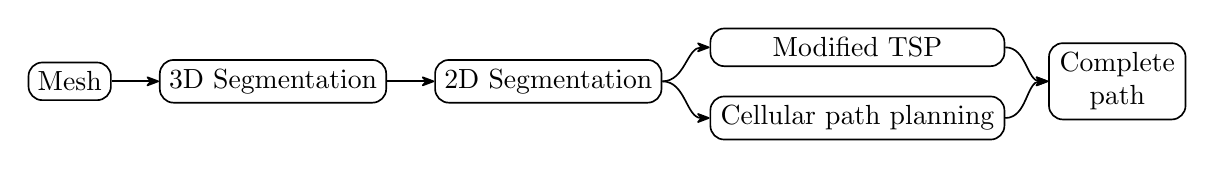
\begin{tikzpicture}[Node/.style={rectangle,semithick,align=center,rounded corners=5pt,draw},
		Arrow/.style={-{Stealth[round]},semithick,out=0,in=180}]
		\pgfmathsetmacro{\dx}{6}
		% nodes
		\node[Node] (Mesh) {Mesh};
		\node[Node] (3DSeg) [right=\dx mm of Mesh] {3D Segmentation};
		\node[Node] (2DSeg) [right=\dx mm of 3DSeg] {2D Segmentation};
		\node[Node,text width=35mm] (TSP) [above right=-1mm and \dx mm of 2DSeg] {Modified TSP};
		\node[Node,text width=35mm] (Bpath) [below right=-1mm and \dx mm of 2DSeg] {Cellular path planning};
		\node[Node,text width=15mm] (Path) [right=49mm of 2DSeg] {Complete path};
		% connections
		\draw [Arrow] (Mesh) -- (3DSeg);
		\draw [Arrow] (3DSeg) -- (2DSeg);
		\draw (2DSeg) edge [Arrow] (TSP);
		\draw (2DSeg) edge [Arrow] (Bpath);
		\draw (TSP) edge[Arrow] (Path);
		\draw (Bpath) edge[Arrow] (Path);
	\end{tikzpicture}
	\caption{Path generation procedure overview}
	\label{fig:procedure_overview}
\end{figure}

Testing is currently conducted using a UR10 from Universal Robots.
During prior testing, commands were sent to the robot without guarantee that the previous command had been fully executed.
Newly received commands would interrupt the current command, leading to jerky, and sometimes erroneous movement.
In order to prevent such issues, XML-RPC was chosen as the communication method between controller and robot for this project \cite{UR_XML-RPC}.
XML-RPC (Remote Procedure Call) is a communication protocol that allows programs to communicate via HTTP independent of OS and architecture.
A cursory examination of the UR programming facilities revealed nothing akin to a queue with which to hold received commands.
As such, queuing of commands will take place server-side (controller) and the robot will be programmed to process commands individually, requesting the next as the current is completed.
The algorithm will be evaluated according to how complete, swift, and collision-free the resultant path is.
To measure path completeness, a spray paint accessory could be attached to the robot arm to paint the test object.
Areas left unpainted count against the path's completeness.
Swiftness includes both calculation time and path traversal time, and can simply be measured in the program.
Path evaluation for collision-free movement will be handled by simple observation.

\section*{Goal}
The goal of this master's thesis is to develop a coverage path planning algorithm able to handle objects of arbitrary geometry.
The algorithm should cover as much of the target surface as is possible.
Communication between the path planner and the robot should be seamless, such that the robot's movements are uninterrupted by path planner communication.

\section*{Task}
\begin{enumerate}
	\item Develop coverage path planning algorithm
	\begin{enumerate}
		\item Develop and implement robust surface segmentation algorithm
		\item Develop or obtain an inverse-kinematic solver to ensure clean robotic movement
		\item Evaluate algorithm using 3D printed test objects
	\end{enumerate}
	\item Communicate with robot via XML-RPC
	\begin{enumerate}
		\item Create a client-side (robot) program to accept and execute commands via XML-RPC
		\item Test connection to a virtual machine
		\item Test connection to a demonstration robot
	\end{enumerate}
	\item Test various sample objects to validate algorithm robustness
	\item Evaluate algorithm on UR3 according to the following criteria:
		\begin{itemize}
			\item collision-free movement
			\item coverage completeness
			\item planning and execution time
		\end{itemize}
\end{enumerate}

\printbibliography
\end{document}
